\begin{figure}[h]
    \centering
    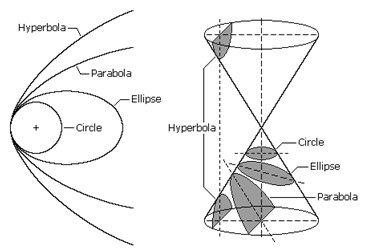
\includegraphics[scale=0.7]{AerospaceApplications/images/orb_dyn.png}
\end{figure}

After the explanation of the main topics about attitude kinematics, dynamics and control, we have to move to something also very important, but different.\\ We have said that a spacecraft can be thought as a rigid body and for this reason, its motion can be described separately in two parts: \textit{rotational motion} in which it is important to define the pshysical quantities in order to describe the attitude, then we study the \textbf{traslational motion} which include the study of the \textbf{orbital dynamics}, here how will be discussed, the presence of the gravitational field is very important.\\

Orbital dynamics is based on \textbf{celestial mechanics} which is composed by a set of equations:
\begin{itemize}
    \itemsep0em
    \item The three \textbf{Kepler's laws} which describe the motion of bodies on orbits in unperturbed system; 
    \item \textbf{Newton's laws} which are more general, moreover using them it is possible to derive the Newton's laws. They are three plus another which is the \textit{law of gravitation}.
\end{itemize}

\section{Fundamental laws}
\subsection{Kepler's laws}
\begin{enumerate}
    \item \textsf{\textbf{First} law}. A planet describes an \textbf{ellyptical orbit}, the sun is located in one of the foci; 
    \item \textsf{\textbf{Second} law}. The radius vector drawn from the sun to any planet sweeps out \textbf{equal areas in equal time}, that is the same to say that the \textbf{aeral velocity} is constant; 
    \item \textsf{\textbf{Third} law}. The \textbf{period of revolution} of a planet is proportional to $r_m^{3/2}$, where $r_m$ is the mean distance of the planet itself from the sun. 
\end{enumerate}

How we mentioned these laws are derived by using other general mechanics laws which are the three Newton's laws + law of gravitation.

\subsection{Newton's laws}
\begin{enumerate}
    \item \textsf{\textbf{First law}}. Unless an \textit{external force} acts, a particle remains at rest or continues to move at a \textbf{constant velocity}
    \footnote[1]{Note that when a particle remains at rest means that its velocity is such that $\mathbf{v}=0$, which is a \textbf{particular case} of constant velocity $\mathbf{v}=\text{const}$}; 
    \item \textsf{\textbf{Second law}}. The linear momentum {\footnote[2]{\textbf{Linear momentum} $\mathbf{p}=m\mathbf{v}$}} changes according to the following equation: 
    \begin{equation*}
        \frac{d}{dt}(m\mathbf{v}) = \textbf{F}
    \end{equation*}
    \begin{align*}
        &m: \quad \text{mass of the particle (could be varible in time)}\\
        &\mathbf{v}: \quad \text{velocity of the particle}\\
        &\mathbf{F}: \quad \text{Force acting on the particle (resultant)}
    \end{align*}
    \item \textsf{\textbf{Third law}} For any force $\mathbf{F}_{12}$ exerted by a particle 1 on a particle 2, there is a force $-\mathbf{F}_{21}$ from the particle 2 to the particle 1, on the same direction, opposite side.
    \item \textsf{\textbf{Law of gravitation}} Given two particles $m_1, m_2$, they attract \textbf{each other} with a force expressed as
    \begin{equation*}
        \mathbf{F} = G\frac{m_1m_2}{r^3}\mathbf{r}
    \end{equation*}
    \begin{align*}
        &m_1, m_2: \quad \text{particle masses}\\
        &\mathbf{r}: \quad  \text{vector of magnitude r which links the particles}\\
        &G: \quad \text{universal constant of gravitation}
    \end{align*}
\end{enumerate}

\section{The two-body problem}\footnote[3]{
    In the following the particle masses are assumed to be constant.
}
Putting together the basic notions we have presented, when you have two particles on which external forces are applied, an interesting problem arises which is the \textbf{two-body problem} on which for centuries scientists have dedicated their studies and efforts. It is extremely important when we are modeling the \textit{orbital dynamics} for aerospace applications, especially for a particular \textbf{restricted form}.\\
Let us consider two masses $m_1, m_2$ located in the positions $P_0$ and $P_1$ in an inertial frame {\footnote[4]{A reference frame with origin $O$ is said to be \textbf{inertial}, if $\dot{\mathbf{v}}=0 \iff \mathbf{v}=\text{const}$}} whose origin is $O$. It is useful to define the following quantities: 
\begin{itemize}
    \itemsep0em
    \item[\ding{202}] $\mathbf{r}_0, \mathbf{r}_1$ are the positions of the particle in the inertial reference frame, while their \textbf{relative position} is: $\mathbf{r}=\mathbf{r}_1-\mathbf{r}_0$;
    \item[\ding{203}]  $\mathbf{v}_0, \mathbf{v}_1$ are the velocities of the particle, equivalently to the positions, the quantity $\mathbf{v}=\mathbf{v}_1-\mathbf{v}_0$ is the \textbf{relative velocity}; 
    \item[\ding{204}] $\mathbf{F}_0$ and $\mathbf{F}_1$ are \textbf{external} (non gravitational) forces which are applied on the single particles.
    \item[\ding{205}] The \textbf{center of mass (CoM)} is characterized by the following quantities:
    \begin{itemize}
        \itemsep0em
        \item[\ding{52}] \textbf{CoM position}: it is the weighted mean of the single positions $$\mathbf{r}_c= \frac{m_0}{m_0+m_1} \mathbf{r}_0 + \frac{m_1}{m_0+m_1} \mathbf{r}_1$$ 
        \item[\ding{52}] \textbf{CoM velocity}: it is the weighted mean of the velocities
        $$
        \mathbf{v}_c = \frac{m_0}{m_0+m_1} \mathbf{v}_0+ \frac{m_1}{m_0+m_1} \mathbf{v}_1
        $$
    \end{itemize} 
\end{itemize}

Using these information, and doing some simple computation, a very important equation will be derived in the following.\\
By using the \textit{II Newton's law} we can write for each of the two bodies the equations: 
\begin{itemize}
    \item[\ding{202}] \textsf{\textbf{Particle $\mathsf{m_0}$}}. \begin{align*}
        m_0 \mathbf{v_0} = \sum{\mathbf{F}_i} &= G\frac{m_0m_1}{r^3}\mathbf{r} + \mathbf{F}_0 \overset{\frac{1}{m_0}}{\iff}\\
        &\mathbf{v_0} = G\frac{m_1}{r^3}\mathbf{r} + \frac{\mathbf{F}_0}{m_0}
    \end{align*}
    \item[\ding{203}] \textsf{\textbf{Particle $\mathsf{m_1}$}}.
    \begin{align*}
        m_1 \mathbf{v_1} = \sum{\mathbf{F}_i} &= -G\frac{m_0m_1}{r^3}\mathbf{r} + \mathbf{F}_0 \overset{\frac{1}{m_1}}{\iff}\\
        &\mathbf{v_1} =- G\frac{m_0}{r^3}\mathbf{r} + \frac{\mathbf{F}_1}{m_1}
    \end{align*}
\end{itemize}
Using the above equations we obtai, respectively, the expression for the \textit{relative velocity} and for the \textit{CoM velocity}.
\begin{align*}
    &\dot{\mathbf{v}}=\dot{\mathbf{v}_1} - \dot{\mathsf{v}_0} =- \frac{G(m_0+m_1)}{r^3}\mathbf{r} + \frac{1}{m_1} \biggl(
        \mathbf{F_1}-\frac{m_1}{m_0}\mathbf{F}_0 
    \biggr) \quad \textsf{(relative motion)}\\
    &\dot{\mathbf{v}}_c = \frac{1}{m_1} \frac{\mathbf{F}_1 + \mathbf{F}_0} {1+m_0/m_1} \quad \textsf{(CoM motion)}
\end{align*}
In some situations the particles $m_0, m_1$ have very different masses{\footnote[5]{ For instance: $m_0$: the Sun, $m_1$: the Earth, or $m_0$: the Earth, $m_1$: a satellite }} that is $m_0 \gg m_1$, then in the first equation above some terms are negligible. In particular, the first becomes:
\begin{equation} \tag{\textsf{2B}} \label{eq: 2B}
    \dot{\mathbf{v}} + \mu \frac{\mathbf{r}}{r^3} = \frac{1}{m_1} \mathbf{F}_1
\end{equation}
where $\mu=Gm_0$ is the \textit{gravitational parameter}. This important equation is called the \textbf{restricted two-body equation}{\footnote[6]{This is a nonlinear ordinary non-homogeneus differential equation, which has attracted the interest from the scientific community for centuries!}}.\\
When $m_0 \gg m_1$ holds, then $\mathbf{\dot{v}}_c=0$, this shows an interesting property: since the CoM has a constant velocity it can be choosen as the \textbf{origin of the inertial reference frame}. The next paragraph is dedicated to the  description of the properties of the equation (\ref{eq: 2B}).
 
\section{Free motion of the restricted two body problem}
It is interesting to study the \textbf{restricted two-body problem} derived from the fundamental laws in the particular case when \textbf{no external forces are applied}, to so-called \textbf{free motion}. The equation \ref{eq: 2B} becomes:
\begin{equation}\tag{\textsf{FR2B}} \label{eq: FR2B}
    \dot{\mathbf{v}} + \mu \frac{\mathbf{r}}{r^3}=0
\end{equation}
Starting from these equation important \textbf{conservation properties} are derived.

\subsection{Energy conservation}
If we make the dot product of the equation (\ref{eq: FR2B}) with $\mathbf{v}$ we obtain:
{\large{
    \begin{align*}
        &\dot{\mathbf{v}} \cdot \mathbf{v} + \mu \frac{\mathbf{r}}{r^3}\cdot \mathbf{v} =
        \frac{1}{2}\frac{d}{dt}(\mathbf{v}\cdot\mathbf{v}) + \frac{\mu}{2r^3}\frac{d}{dt}(\mathbf{r}\cdot\mathbf{r}) \underset{\frac{d}{dt}(r^2)=2r\frac{d}{dt}(r)=2r\cdot\dot{r}}{=}\\ 
        &\frac{d}{dt}\frac{v^2}{2} + \frac{\mu\dot{r}}{r^2} =\frac{d}{dt}\biggl(
            \frac{v^2}{2} - \frac{\mu}{r}
        \biggr) = \dot{\mathcal{E}}=0
    \end{align*}
}}
\noindent
We have proven that the physical quantity
\begin{equation*}
    \mathcal{E} = \frac{v^2}{2} - \frac{\mu}{r}
\end{equation*}
which is the \textbf{mechanical energy per unit mass}\footnote[7]{It is composed of two contributions: (i) \textbf{kinetic energy per unit of mass $\frac{v^2}{2}$}, (ii) \textbf{potential energy per unit of mass} $-\frac{\mu}{r}$ } is constant. For a given (total) energy $\mathcal{E}$ the orbital velocity is given by $v=\sqrt{2\mu/r+2\mathcal{E}}$

\subsection{Angular momentum conservation and planar motion}
Now let us the take the \textit{cross product} of the equation \ref{eq: FR2B} with $\mathbf{r}$ and we will obtain:
{\large{
    \begin{align*}
        &\mathbf{r} \times\dot{\mathbf{v}} + 
        \frac{\mu}{r^3}\mathbf{r} \times \mathbf{r} \overset{r\times r=0}{=} 
        \mathbf{r} \times\dot{\mathbf{v}} =\\
        & \mathbf{v} \times \mathbf{v} + \mathbf{r} \times\dot{\mathbf{v}} = \frac{d}{dt} (\mathbf{r} \times\mathbf{v})=0
    \end{align*}
}}
This proves that the quantity
\begin{equation*}
    \mathbf{h} = \mathbf{r} \times\mathbf{v}
\end{equation*}
the \textbf{angular momentum per unit of mass}, is constant since is derivative is null. Since $\mathbf{h}$ is the cross product between $\mathbf{r}$ and $\mathbf{v}$, it is orthogonal to the plane generated by $\mathbf{r}$ and $\mathbf{v}$, and since the angular momentum is constant, we have also proven that \textbf{the motion occurs on a plane} (which contains the orbit).

\subsection{Orbit equation (ORE)}
Let us take the cross product of the equation \ref{eq: FR2B} with the angular momentum $\mathbf{h}$ and we obtain the following result:
{\large{
    \begin{align*}
        \biggl(
            \dot{\mathbf{v}} +  \frac{\mu}{r^3}\mathbf{r}
        \biggr) \times \mathbf{h} = 
        \frac{d}{dt}\biggl(
            \mathbf{v} \times \mathbf{h} - \frac{\mu}{r}\mathbf{r}
        \biggr)=0
    \end{align*}
}}
The proof
\footnote[8]{Proof of the equality: \begin{align*}
    &\frac{d}{dt}(\mathbf{v}\times\mathbf{h}) = \dot{\mathbf{v}}\times\mathbf{h} + \mathbf{v} \times \dot{\mathbf{h}}= \mathbf{\dot{v}} \times \mathbf{h} \quad (\dot{\mathbf{h}}=0) \\
    &\frac{d}{dt}\biggl(
        -\frac{\mathbf{r}}{r}
    \biggr) = \frac{\dot{r}}{r^2} \mathbf{r} - \frac{1}{r}\mathbf{v} = \frac{1}{2r^3}\biggl(
        \frac{d}{dt} r^2
    \biggr) \mathbf{r} - \frac{1}{r}\mathbf{v} = \frac{1}{2r^3}\biggl(
        \frac{d}{dt} (\mathbf{r} \times \mathbf{r})
    \biggr) \mathbf{r} - \frac{1}{r}\mathbf{v}=\\
    &\frac{1}{r^3} ((\mathbf{r} \cdot \mathbf{v})\mathbf{r}-(\mathbf{r} \cdot \mathbf{v})\times \mathbf{v}=\frac{1}{r^3}\mathbf{r}\times(\mathbf{r}\times\mathbf{v}))=\frac{1}{r^3}\mathbf{r}\times\mathbf{h} \quad (\textsf{vector triple product})
\end{align*}}
of these first equality is based on simple manipulations which exploit some algebraic properties.
The above equation tells us that the quantity
$$
\mathbf{v} \times \mathbf{h} - \frac{\mu}{r}\mathbf{r}=\text{const} \doteq \mu\mathbf{e}
$$
where $\mathbf{e}$ is the \textit{eccentricity vector} and its norm $e=\vert \mathbf{e} \vert$ is called the \textit{eccentricity}. Let us take the dot product of r with the equation we have just derived:
\begin{align*}
    &\mathbf{r}\cdot (\mathbf{v} \times \mathbf{h}) - \frac{\mu}{r}\mathbf{r}\cdot\mathbf{r}=\mu\mathbf{r}\cdot\mathbf{e} \underset{\mathbf{r}\cdot (\mathbf{v} \times \mathbf{h})=(\mathbf{r}\times\mathbf{v})\cdot \mathbf{h}}{\iff} 
    (\mathbf{r}\times\mathbf{v})\cdot \mathbf{h} - \frac{\mu}{r}\mathbf{r}\cdot\mathbf{r}=\mu\mathbf{r}\cdot\mathbf{e}\iff\\
    &h^2 - \mu r = \mu \ r \ e \cos\theta \iff 
    h^2 = \mu \ r \ e \cos\theta + \mu r = \mu r(1+e \ \cos\theta)
\end{align*}
where $\theta$ is the angle between the relative position and the eccentricity vector and it is called the \textit{true anomaly}. By using this latest calculation, by expliciting the last step with respect to $r$ we obtain, given $p=h^2/\mu$ the so-called \textbf{semilatus rectum} or \textbf{parameter}:
{\large{
    \begin{equation} \tag{\textsf{ORE}} \label{eq:ORE}
        r = \frac{p}{1+e \cos\theta}
    \end{equation}
}}
this is the so-called \textbf{orbit equation}.


\section{Orbit geometry}